\documentclass[crop, tikz]{standalone}

\usepackage{tikz}
\usepackage{amsmath}
\usepackage{amssymb}
\usepackage[mode=buildnew]{standalone}

\usepackage{xcolor}


\usetikzlibrary{positioning}
\usetikzlibrary{calc}
\usetikzlibrary{fit}
%\usepackage{nicematrix}

\tikzset{set/.style={draw,circle,inner sep=0pt,align=center}}

\definecolor{morange}{RGB}{255,127,14}
\definecolor{mblue}{RGB}{31,119,180}
\definecolor{mred}{RGB}{214,39,40}
\definecolor{mpurple}{RGB}{148,103,189}
\definecolor{mgreen}{RGB}{44,160,44}


\begin{document}
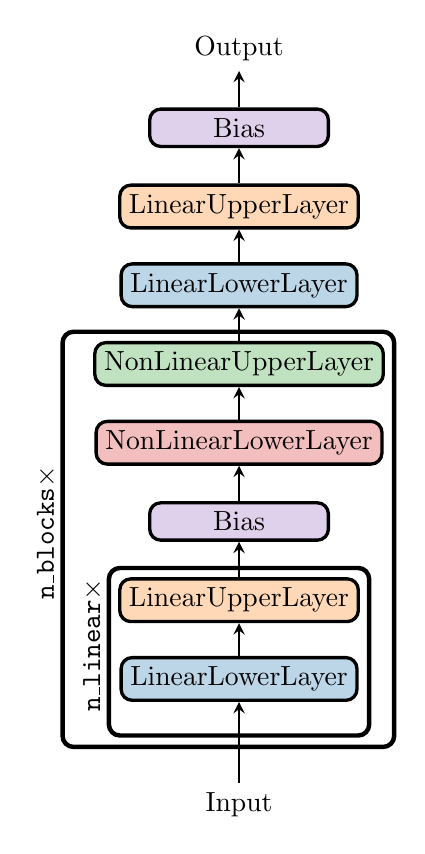
\begin{tikzpicture}[module/.style={draw, very thick, rounded corners, minimum width=15ex},
    linup/.style={module, fill=morange!30},
    linlow/.style={module, fill=mblue!30},
    bias/.style={module, fill=mpurple!30},
    nonlinup/.style={module, fill=mgreen!30},
    nonlinlow/.style={module, fill=mred!30},
    arrow/.style={-stealth, thick, rounded corners},
]
\node (input) {Input};
\node[above of=input, linlow, align=center, yshift=.6cm] (linlow1) {LinearLowerLayer};
\node[above of=linlow1, linup, align=center] (linup1) {LinearUpperLayer};
\node[above of=linup1, bias, align=center] (bias1) {Bias};
\node[above of=bias1, nonlinlow, align=center] (nonlinlow) {NonLinearLowerLayer};
\node[above of=nonlinlow, nonlinup, align=center] (nonlinup) {NonLinearUpperLayer};
\node[above of=nonlinup, linlow, align=center] (linlow2) {LinearLowerLayer};
\node[above of=linlow2, linup, align=center] (linup2) {LinearUpperLayer};
\node[above of=linup2, bias, align=center] (bias2) {Bias};
\node[above of=bias2] (output) {Output};

\draw[arrow] (input) -- (linlow1);
\draw[arrow] (linlow1) -- (linup1); 
\draw[arrow] (linup1) -- (bias1);
\draw[arrow] (bias1) -- (nonlinlow); 
\draw[arrow] (nonlinlow) -- (nonlinup);
\draw[arrow] (nonlinup) -- (linlow2); 
\draw[arrow] (linlow2) -- (linup2); 
\draw[arrow] (linup2) -- (bias2);
\draw[arrow] (bias2) -- (output);

\coordinate (linear_layer_center) at ($(linlow1.north)!0.5!(linup1.south)$);
\coordinate (before_linear_lower_layer) at ($(input.north)!0.7!(linlow1.south)$);
\node[left of=linear_layer_center, xshift=-1cm] (first_label) {};

\node[fit=(before_linear_lower_layer)(linlow1)(linup1),draw, ultra thick, rounded corners, label={[rotate=90, yshift=.5em, xshift=3em]left:$\mathtt{n\_linear}\times$}] (linear) {};
\node[fit=(linear)(bias1)(nonlinlow)(nonlinup)(first_label), draw, ultra thick, rounded corners, label={[rotate=90, yshift=.5em, xshift=3em]left:$\mathtt{n\_blocks}\times$}] (block) {};
\end{tikzpicture}
\end{document}